\documentclass[12pt]{article}

% \usepackage[utf8]{inputenc}
\usepackage[T1]{fontenc}
\usepackage[francais]{babel}
%Options: Sonny, Lenny, Glenn, Conny, Rejne, Bjarne, Bjornstrup
% \usepackage[Lenny]{fncychap}
% \usepackage{mathpazo}
\usepackage{fontspec}
\setmainfont{ubuntu}
\usepackage[a4paper, width=150mm, top=25mm, bottom=25mm]{geometry}
\usepackage[colorlinks=true, linkcolor=blue, unicode]{hyperref}
\frenchbsetup{StandardLists=true}
\usepackage{enumitem}
\setlist[itemize]{label=\textbullet, topsep=0cm}
\setlist[description]{topsep=0cm}
\usepackage{parskip}
\usepackage{graphicx}
\usepackage{float}
\usepackage[bottom]{footmisc}
\usepackage[defaultlines=4,all]{nowidow}
\usepackage{subcaption}
\usepackage{array}

% To write inline code.
\usepackage{xcolor}
\definecolor{light-gray}{gray}{0.90}
\newcommand{\code}[1]{\colorbox{light-gray}{\texttt{#1}}}

\usepackage{listings}

\lstdefinestyle{code}{
language=python,                   
keywordstyle=\color{blue},      
stringstyle=\color{red},        
commentstyle=\color{gray},     
basicstyle=\small\ttfamily,           
numbers=left,                   
numberstyle=\normalsize,        
numbersep=7pt,                  
showstringspaces=false,         
breaklines=true,                
frame=leftline,                 
framerule=2pt,
}

\lstdefinestyle{exec_result}{
frame=tb,
language=bash,
aboveskip=3mm,
belowskip=3mm,
showstringspaces=false,
columns=flexible,
basicstyle={\small\ttfamily},
numbers=none,
numberstyle=\tiny\color{gray},
breaklines=true,
breakatwhitespace=true,
framerule=2pt,
}


\usepackage{awesomebox}
\def\abIconQuestion{\symbol{"F059}}
\newcommand{\questionbox}[1]{%
  \awesomebox{\abIconQuestion}{\aweboxrulewidth}{abwarning}{#1}}

\begin{document}
\pagenumbering{gobble}
\renewcommand{\contentsname}{Sommaire}
\tableofcontents
\newpage

\pagenumbering{arabic}

\section{La programmation avec Python 3}
    \subsection{Introduction}
        Ceci est une petite introduction où on va parler des programmes et des langages de programmations.
        \subsubsection{C'est quoi un programme ??}
            Je vais commencer par donner une définition qui peut vous semblez un peu floue, mais cette description
            va s'éclaircir coûte que coûte au cours de notre formation. 

            Alors, un programme est un ensemble d'instructions exécuté par l'ordinateur pour qu'il puisse (l'ordinateur)
            accomplir une tâche bien précise. On a pour exemple des programmes : les navigateurs web 
            (comme chromium, chrome, firefox), qui permettent de visiter les cites et de chatter en ligne ;
            on a aussi les jeux vidéos, les logiciels de retouches de photos \ldots\ etc

            \begin{figure}[H]
                \centering
                \begin{subfigure}[b]{0.49\textwidth}
                    \centering
                    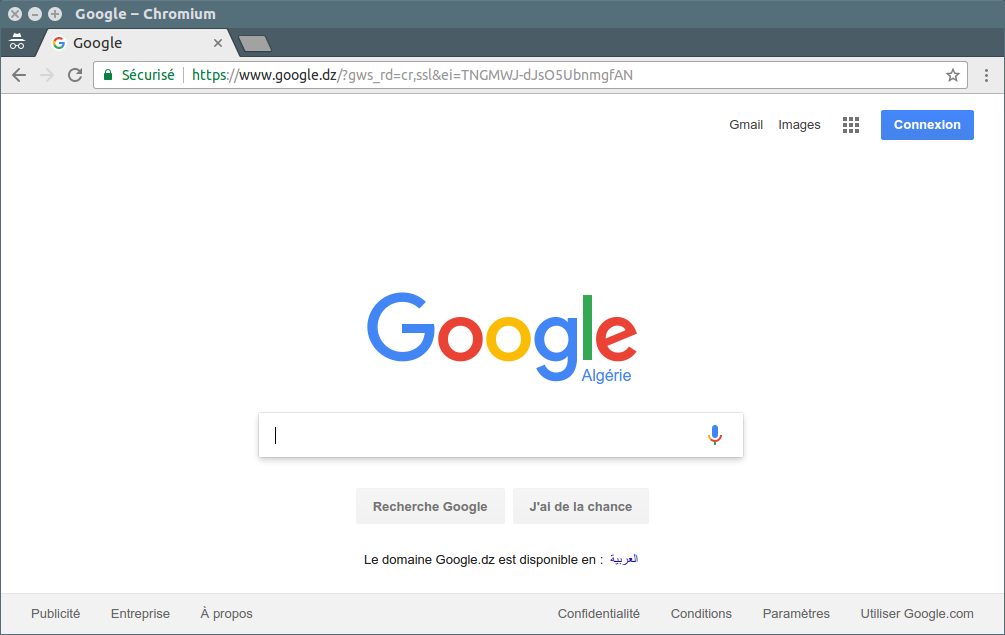
\includegraphics[width=\textwidth, height=2in]{img/1_chrome.png}
                    \caption{Google Chrome}
                \end{subfigure}
                \hfill
                \begin{subfigure}[b]{0.49\textwidth}
                    \centering
                    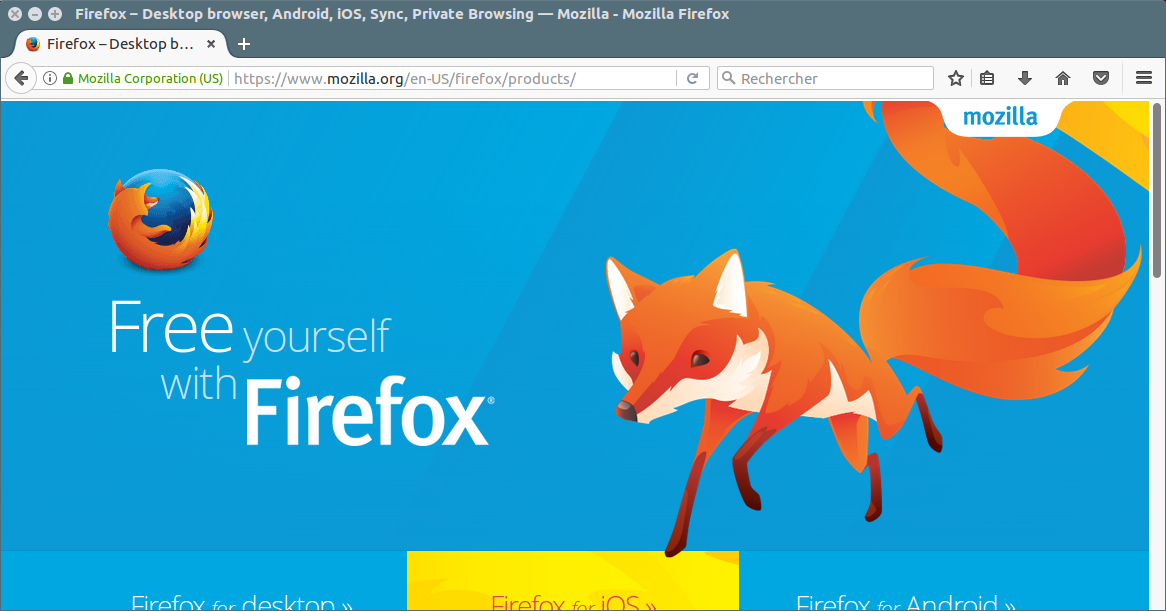
\includegraphics[width=\textwidth, height=2in]{img/2_firefox.png}
                    \caption{Mozilla Firefox}
                \end{subfigure}
            \end{figure}

            \begin{figure}[H]
                \centering
                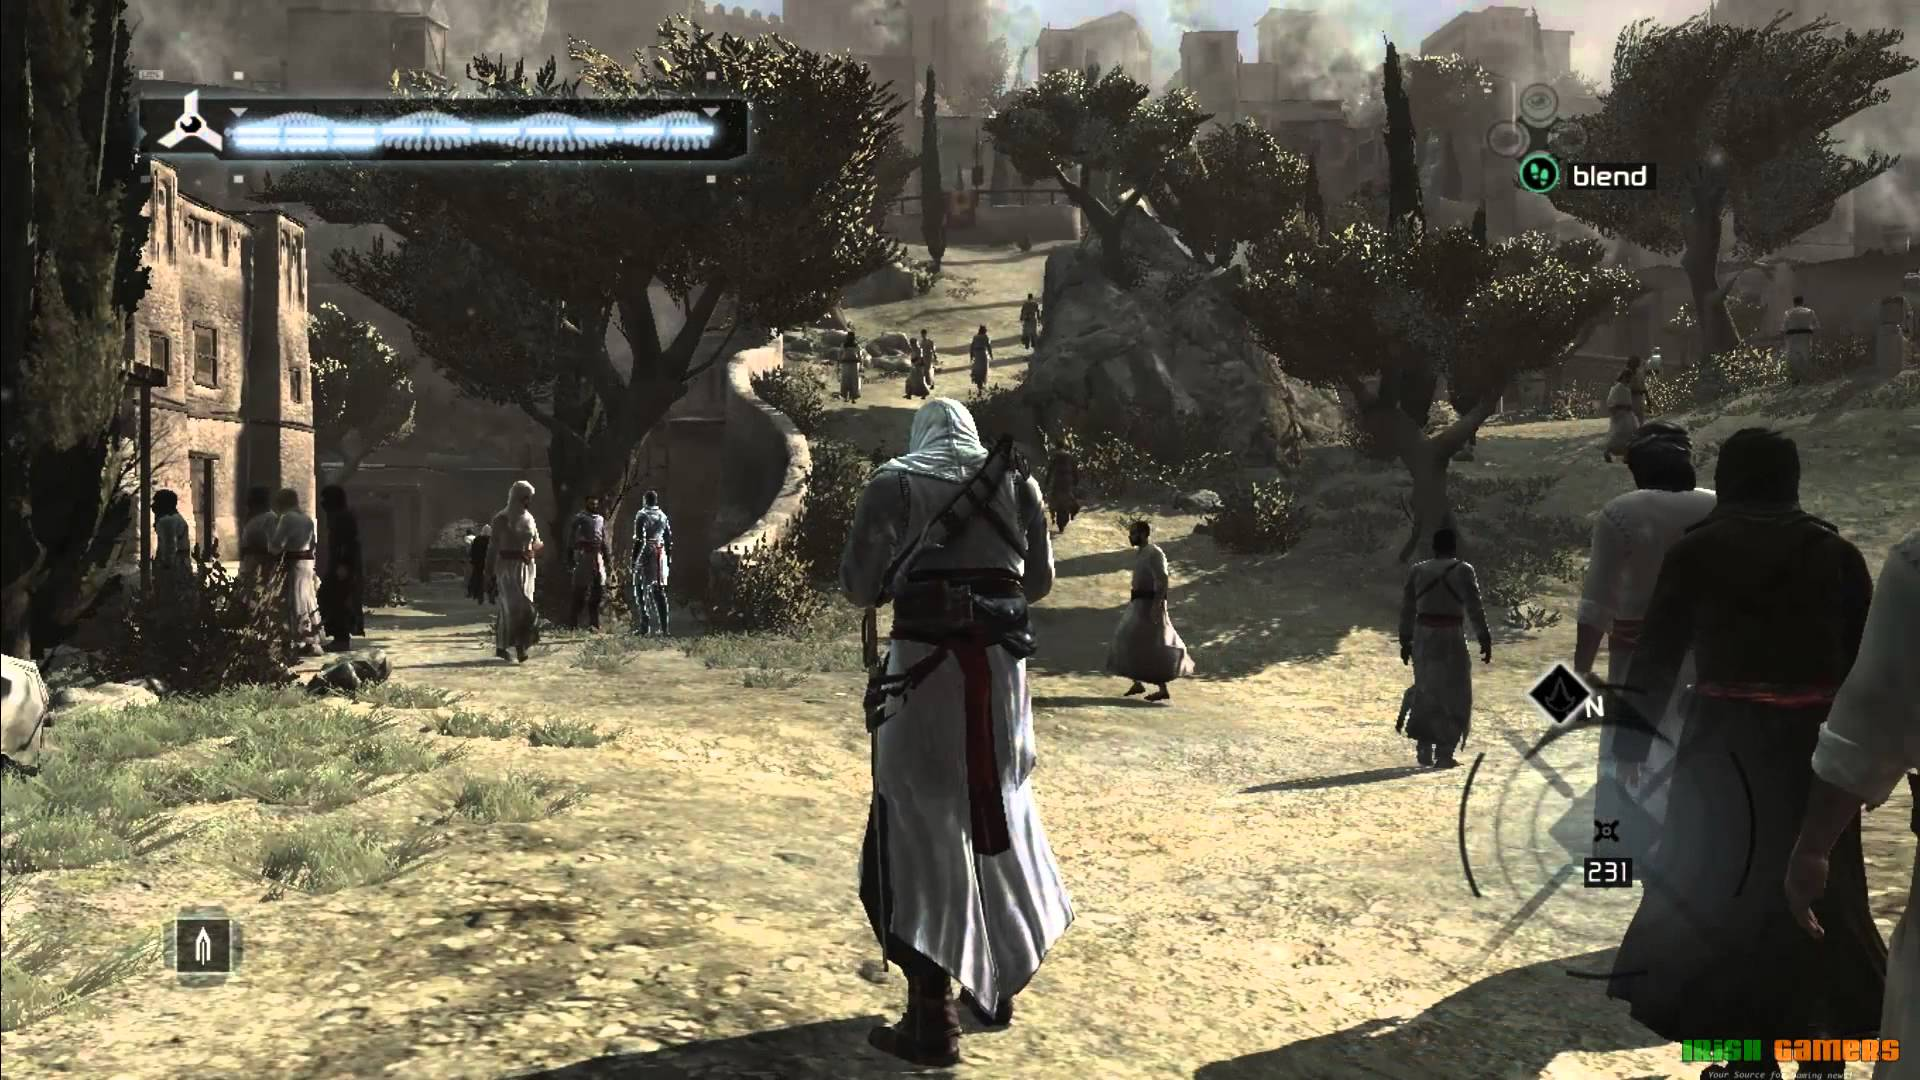
\includegraphics[width=\textwidth]{img/3_assassins_creed.jpg}
                \caption{Le jeu Assassin's Creed}
            \end{figure}
            \begin{figure}[H]
                \centering
                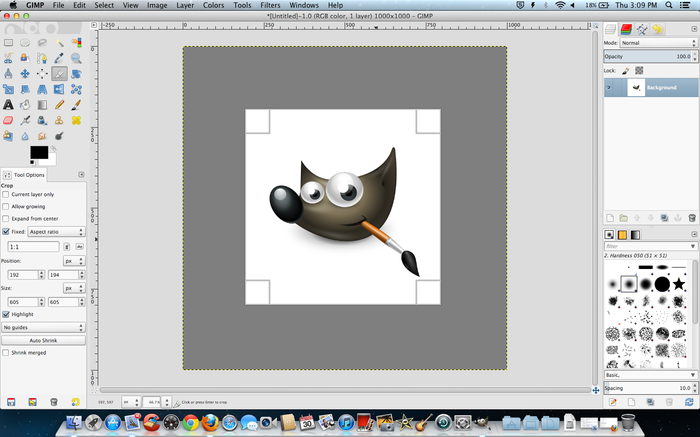
\includegraphics[width=\textwidth]{img/4_gimp.png}
                \caption{Logiciels de retouches ``Gimp''}
            \end{figure}
            % Dans tous les exemples citer avant, on voit que ces programme
            % demande à l'ordinateur d'exécuter des instructions pour qu'il puisse servir; tous ces programmes donnent des instructions bien précise à
            % l'ordinateur pour qu'il puisse accomplir certaines tâches

        \subsubsection{Comment sont crée ces programmes ??}
            L'ordinateur est une machine bête et discipliné qui ne comprend qu'un seul langage, qui est le langage
            \emph{binaire}. Ce langage est une succession de 1 et de 0 comme suit : 
            \begin{lstlisting}[style=code,numbers=none]
01101100001100110011000111101011101
            \end{lstlisting}
            
            Donc, normalement, pour créer des programmes, il fallait apprendre ce langage.
            Mais heureusement, les informaticiens ont eu la réflexion de créer d'autres langages intermédiaires 
            (qu'on appel langage de programmation) qui sont beaucoup plus facile que le binaire. Ces langage ont 
            tous le même but : permettre de créer des programmes plus facilement qu'en binaire.
            
            Voici comment cela fonctionne :
            \begin{itemize}
                \item On donne nos instructions à l'ordinateur en utilisant un langage de programmation.
                \item Les instructions sont traduites en binaire grâce à un programme de traduction.
                \item L'ordinateur peut alors lire le binaire et faire ce qu'on l'a demandé.
            \end{itemize}

            Voici une image qui illustre ce qu'on vient de dire :
            \begin{figure}[H]
                \centering
                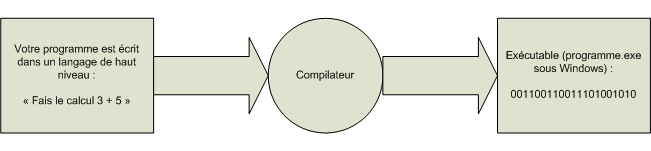
\includegraphics[width=\linewidth]{img/11_compilation.png}
                \caption{Les étapes de création d'un programme}
            \end{figure}

            Une remarque très importante : les instructions que nous écrivons dans un langage de programmation 
            sont appelé \textbf{Code Source}. Gardez bien ce terme à l'esprit, parce qu'on va beaucoup l'utiliser 
            par la suite. Voici un exemple de code source python que nous écrirons plus tard :
            
            \begin{figure}[H]
                \centering
                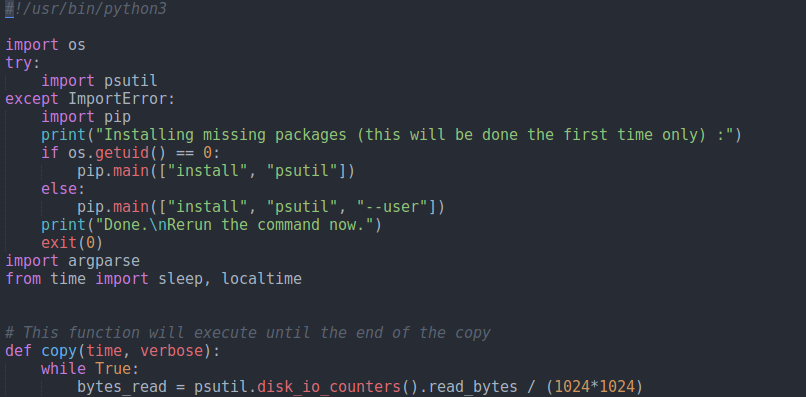
\includegraphics[width=\linewidth]{img/12_code.png}
                \caption{Coude source Python}
            \end{figure}

        \subsubsection{Les langages de programmation les plus connus}
            \begin{description}
                \item[C++ :] La formation est faite par \textsc{Yasser}.
                \item[Java :] La formation est faite par \textsc{Wissam} et \textsc{Sofiane}.
                \item[Python :] C'est la formation à laquelle vous assistez maintenant.
            \end{description}

        \begin{figure}[H]
            \centering
            \begin{subfigure}[b]{0.32\textwidth}
                \centering
                
\includegraphics[width=\textwidth]{img/5_c++.png}
                \caption{Logo C++}
            \end{subfigure}
            \hfill
            \begin{subfigure}[b]{0.32\textwidth}
                \centering
                
\includegraphics[width=\textwidth]{img/6_java.png}
                \caption{Logo Java}
            \end{subfigure}
            \hfill
            \begin{subfigure}[b]{0.32\textwidth}
                \centering
                
\includegraphics[width=\textwidth]{img/7_python.png}
                \caption{Logo Python}
            \end{subfigure}
        \end{figure}
       
        \subsubsection{Compilé vs Interprété}
            Nous avons dit tout à l'heure que les instructions sont traduites en binaire pour que l'ordinateur puisse
            les comprendre et les exécuter. Mais ce qu'on a pas dit c'est qu'il y a deux façons de traduire 
            les instructions : \emph{Compilation} et \emph{Interprétation}.

            \begin{description}
                \item[Compilation :] Avec ce processus, toutes nos instructions sont traduites en binaires à la fois.
                    Ce qui nous donne en résultat un gros fichier binaire qui peut être exécuté directement par
                    l'ordinateur.
                \item[Interprétation :] Avec cette technique, on ne traduit pas tous les instructions en binaires, mais
                    on va plutôt traduire une instruction par instruction à chaque fois qu'on veut exécuter 
                    notre programme. Par exemple, si mon code source contient 3 instructions, quand je veux l'exécuter je
                    traduit la première instruction en binaire, et je la passe à l'ordinateur pour qu'il l'exécute ;
                    ensuite je traduit la deuxième instructions, et je la passe à l'ordinateur pour qu'il l'exécute
                    \ldots\ et ainsi de suite jusqu'à la traduction de toute
                    mes instructions.

                    Le programme qui fait l'interprétation est appelé l'\emph{interpréteur}, et dans notre cas on va utiliser
                    l'interpréteur \emph{Python}.
            \end{description}

        \subsubsection{Le langage Python}
            Python est un langage de programmation interprété, \emph{Open Source}, facile à apprendre, 
            et très pratique. On cite quelques avantages de ce langage :
            \begin{itemize}
                \item Python est facile à apprendre et son code est facile à lire.
                \item Il est multiplate-forme, il marche sous Linux, Windows, et Mac OS.
                \item C'est un langage orienté objet (on en parlera de ça dans le prochaines séances).
                \item Il a une bibliothèque tierce qui permet de faire de la programmation web d'une manière très flexible.
                    Cette bibliothèque c'est \emph{Django}.
                \item Il permet de développer très rapidement en utilisant peu de code, et de crée des applications 
                    très complexe avec facilité. Tous ça grâce à son style et à sa bibliothèque standard très complète.
            \end{itemize}

            Pour finir, il faut savoir que les géants de l'informatique comme Google, Yahoo, NASA préférent le langage
            python ; et ce langage est intégré à la quasi totalité des distributions Linux (C'est-à-dire que vous pouvez l'utiliser
            dans ces distributions sans devoir l'installer).

            \notebox{
            Juste pour information, il en existe deux versions de python qui ne sont pas compatibles entres eux. Ces
            deux versions sont les 2.x et les 3.x . Nous on va utiliser la version 3.x qui est le future de python.}
            % \subsubsection{Les versions de Python}
            %     Python a deux versions qui ne sont pas compatibles entres eux. Ces deux versions sont la version \emph{2.x}
            %     et \emph{3.x}. La version 2.x n'est plus en développement, et il a été pour des raisons de compatibilité
            %     seulement (pour que les anciens programmes écrit en python 2.x continue à fonctionner sans problème).

    \subsection{Les logiciels nécessaires pour la programmation}
        Pour pouvoir créer des programmes en python, il existe deux manières :
        \begin{enumerate}
            \item Soit on écrit nos instructions dans un fichier texte, et puis on appel l'interpréteur python pour
                qu'il exécute nos instructions et nous affiche le résultat. Cette méthode comporte de nombreux
                avantages, et elle très flexible, mais elle est compliqué (surtout pour les débutants). Donc nous 
                allons optez pour la deuxième méthode dans cette formation.
            \item Cette méthode consiste à utiliser un programme appelé \emph{IDE} (Integrated Development Environment),
                ou \emph{EDI} en français (Environnement de Développement Intégré). Ce programme contient tous ce dont 
                on a besoin pour créer nos programmes : une partie ou on peut écrire nos instructions, des boutons
                pour demander à python d'exécuter nos instructions, et finalement une partie ou le résultat de 
                l'exécution est affiché.
        \end{enumerate}

        L'IDE qu'on va utiliser est appelé \emph{PyCharm} (\autoref{pycharm}). C'est un IDE \emph{Open Source} et très 
        puissant.
        
        \begin{figure}[H]
            \centering
            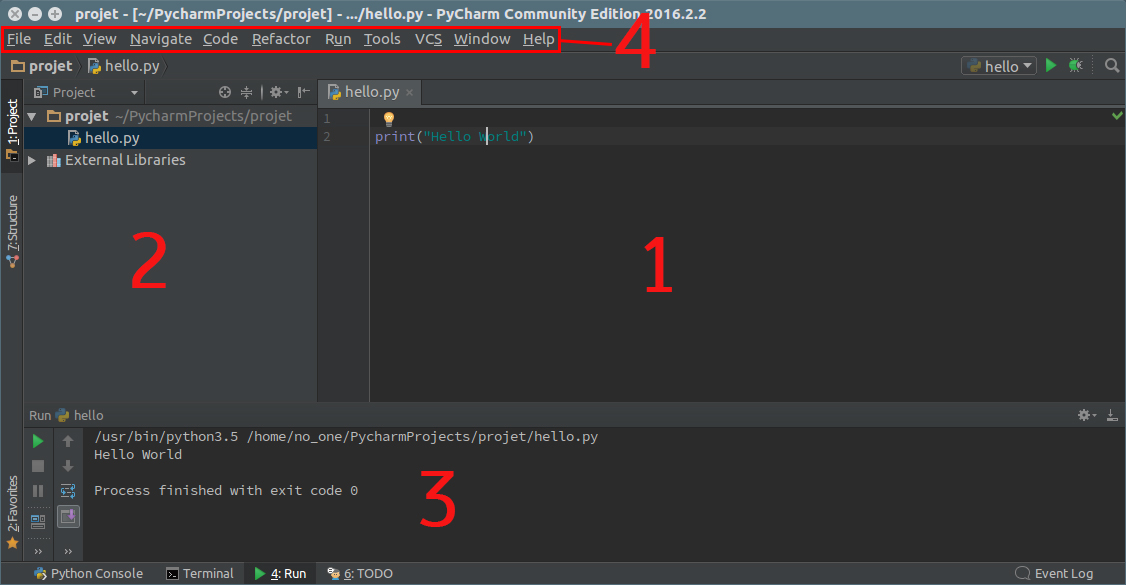
\includegraphics[width=\linewidth]{img/8_pycharm.png}
            \caption{Pycharm}
            \label{pycharm}
        \end{figure}

        PyCharm est composé essentiellement de 4 partie :
        \begin{description}
            \item[La zone principale (1):] c'est dans cette zone où on écrira notre code source (nos instructions).
            \item[La liste des fichiers du projet (2):] dans cette zone on peu voir tous les fichiers de notre projet. 
                On voit bien que le projet présenté dans la \autoref{pycharm} contient un seul fichier seulement.
            \item[La zone d'affichage (3):] c'est cette zone qui nous affichera le résultat d'exécution de notre 
                programme, où les éventuelles erreurs s'il y en a.
            \item[La barre d'outils (4):] elle contient de nombreux boutons qui font différentes choses : exécuter 
            le projet, configurer l'IDE \ldots\ etc, mais nous on utilisera que quelques boutons.
        \end{description}

\clearpage

    \subsection{Hello World}
        Nous allons écrire maintenant notre premier programme. Un programme petit et simple pour comprendre le 
        fonctionnement de ce langage fascinant.

        On commence par créer un nouveau projet en cliquant sur la barre d'outils sur \code{File -> New Project}. Ensuite on choisis où on veut placer notre projet, et la version de l'interpréteur qu'on veut utiliser
        (\autoref{pycharm_new_project}). Choisissez n'importe quelle version 3.x disponible sur votre ordinateur
        (Pour moi, j'utilise la version 3.5).

        \begin{figure}[H]
            \centering
            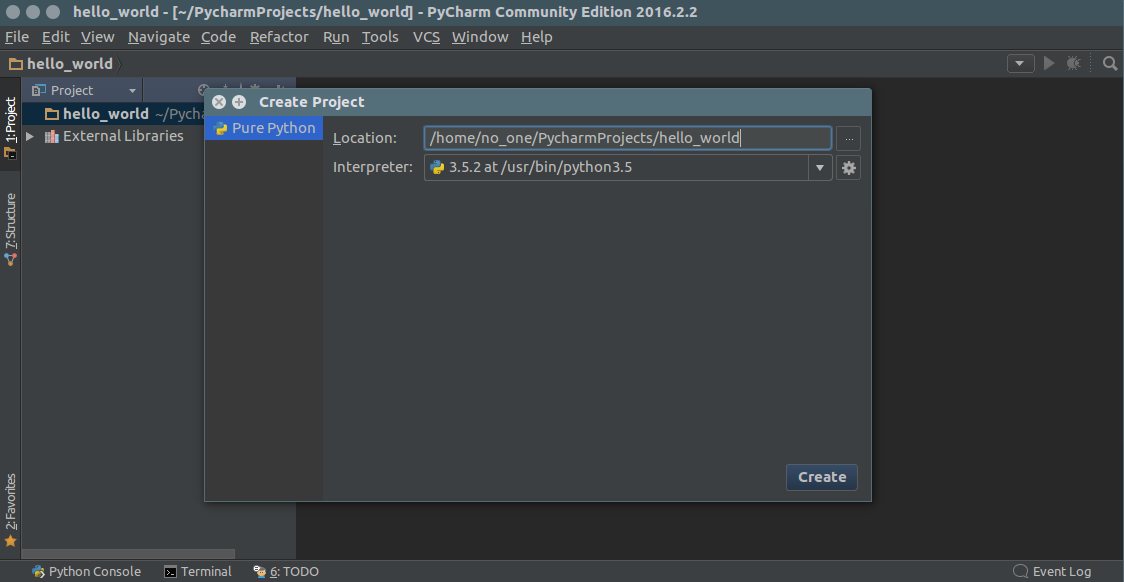
\includegraphics[width=\linewidth]{img/9_new_project.png}
            \caption{Création d'un nouveau projet}
            \label{pycharm_new_project}
        \end{figure}

        On a crée notre projet, mais ce dernier est vide, il ne contient aucun fichier. Nous allons maintenant ajouter
        un fichier où nous allons écrire nos instructions (programmes). On fait un clique sur la barre d'outils sur
        \code{File -> New} et on choisit \code{Python File}. On lui donne un nom à notre fichier, et on clique sur 
        \code{OK} (\autoref{new_file}).

        \begin{figure}[H]
            \centering
            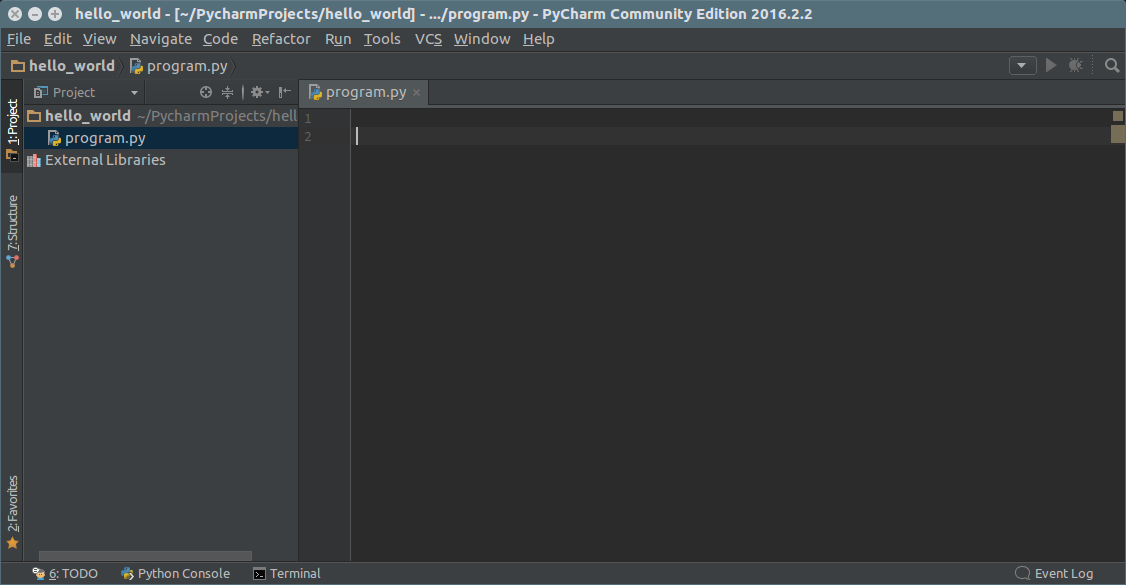
\includegraphics[width=\linewidth]{img/10_new_file.png}
            \caption{Création d'un fichier pour écrire les instructions}
            \label{new_file}
        \end{figure}

        Dorénavant, je vais seulement vous affiché les codes que vous devez écrire dans la zone principale (la zone 
        \textbf{1}, \autoref{pycharm}).

        On arrive maintenant à la programmation, voici votre premier programme :
        \begin{lstlisting}[style=code]
print("Hello World!")
        \end{lstlisting}

        Écrivez ce code source dans la zone principale (zone \no1 \autoref{pycharm}), et demandez à PyCharm 
        d'exécuter notre programme en cliquant sur la barre d'outils sur \code{Run -> Run}, et on choisit le fichier
        à exécuter (on en a un seul dans notre cas). Voici le résultat de l'exécution :

        \begin{lstlisting}[style=exec_result]
/usr/bin/python3.5 /home/no_one/PycharmProjects/hello_world/program.py
Hello World!

Process finished with exit code 0
        \end{lstlisting}

        Alors, la ligne que nous avons écrit dans l'IDE \code{print("Hello World!")} est une instruction qui demande
        à l'ordinateur d'afficher \code{Hello World!} à l'écran. Nous pouvons écrire n'importe quoi à la place de 
        \code{Hello World!} et l'ordinateur se chargera d'afficher le message que nous avons demandé. 
        
        Avant de continuer, nous allons détaillé ce que PyCharm nous a affiché :
        \begin{description}
            \item[/usr/bin/python3.5] c'est le chemin vers l'interpréteur python que PyCharm a utilisé pour 
                exécuté notre programme. La majorité des programmes sous \emph{Linux} sont installés dans le dossier 
                \code{/usr/bin/}\ .
            \item[/home/no\_one/PycharmProjects/hello\_world/program.py] ça c'est notre fichier (là où on est entrain 
                d'écrire notre code source). Donc d'après cette ligne, on comprend que \code{python3.5} est entrain
                d'exécuter ce fichier.
            \item[Hello World!] c'est le message que nous avons demandé à python d'affiché (on voit qu'il a bien 
                obéi).
            \item[Process finished with exit code 0] ceci est un message affiché par \code{PyCharm} pour nous indiquer
                que notre programme s'est terminé avec succès.  
        \end{description}

        Donc, \code{print()} est l'instruction responsable d'afficher un message à l'écran. On lui donne entre 
        les \code{""} le message qu'on veut afficher.
        Essayez de Remplacer \code{Hello World!} par \code{Salut tout le monde} et ré-exécuté pour voir le nouveau résultat. 

        \subsubsection{Les commentaires}
            Avant de terminer cette section avec un TP, nous allons parler des commentaires. 
            Dans n'importe quel langage de programmation (y compris python), on a la possibilité d'écrire des commentaires.

            Alors c'est quoi les commentaires ? Ce sont des bouts de textes qu'on écrit dans notre code source et qui
            permettrons d'expliquer le fonctionnement de notre code source. Ça peut vous semblez bizarre et inutile, mais
            sachez que c'est très commun qu'on revient à notre programme après quelques semaines pour l'améliorer 
            ou pour le modifier, et sans les commentaires on sera obligé de tout repenser du début. Ne vous faites pas 
            avoir par le fait que c'est vous qui a crée ce programme, car même si vous comprenez tous sur votre
            programme maintenant, vous oublierai après un certain temps.

            Les commentaires ne serviront pas seulement à comprendre son code seulement, mais c'est très utile aussi
            quand vous travaillez en groupe pour crée un programme. Quand vous utilisez les commentaires, vous ne serrez
            pas obligé d'expliquer la partie que vous avez écrit à vos camarades.
            
            J'insiste exprès sur le fait d'utiliser les commentaires, ils sont très très utiles et indispensables.

            Alors, on sait ce que sont les commentaires, mais comment les utiliser avec \code{python} ? Voici 
            un exemple sans plus tardé :
            \begin{lstlisting}[style=code]
# Cette instructions affiche Hello World! a l'ecran.
print("Hello World!") 
            \end{lstlisting}

            Les commentaires commence par un \code{\#}, tous ce qui suit ce caractère est ignoré par \code{python}.
            Donc on peut écrire autant de ligne de commentaire qu'on veut, il faut juste précédé chaque ligne avec un
            \code{\#}.

        \subsubsection{Exercice 1}
            Bon, on a assez bavardé, vous allez écrire votre vrai premier programme crée par vous même.
            Voici l'exercice :
            \begin{itemize}
                \item Créez un nouveau projet et nommé le ``exercice 1''.
                \item Créez un fichier dans ce projet où nous allons mettre notre code source. nommé ce fichier
                    ``main''.
                \item Débrouillez vous pour que le programme affiche :
                    \begin{lstlisting}[style=exec_result, breaklines=false]
Salut tout le monde.
On est dans une formation python, et on va cree des programmes super cool :D.
                    \end{lstlisting}
                \item N'oubliez pas d'utiliser les commentaires pour expliquer votre code.
            \end{itemize}

        \subsubsection{Solution de l'exercice}
            \begin{lstlisting}[style=code, breaklines=false]
# Ces deux instructions affiche des messages a l'ecran.
print("Salut tout le monde.")
print("On est dans une formation python, et on va cree des programmes super cool :D.")
            \end{lstlisting}

\clearpage

    \subsection{Les variables}
        Les variables sont une notion fondamentale en informatique et il sont utilisé dans tous les langages
        de programmation sans exception. Il ont plusieurs définitions, mais je pense que celle qu'on va voir est la plus simple.

        En faite, votre ordinateur est une armoire géante qui contient des millions et des millions de tiroirs, et
        chaque tiroir 
        est utilisé pour stocker des informations. Donc quand vous voulez stocké une information (disons votre age) 
        pour l'utilisé plus tard dans votre programme, vous demandez à votre ordinateur de vous allouer un tiroir. 
        Ce tiroir vous serra allouer jusqu'à la fin de votre programme.

        \colorbox{red}{Photos ici avec un tiroir avec la valeur 20 dedans}

        Ce tiroir est le votre, vous pouvez placez des information dedans, les consulter, les retirer.


        Donc, où sont les variables dans tous ça ?? Les variables sont des noms qu'on associé aux tiroirs que nous 
        avons demandé. Donc, dans l'exemple précédent, nous avons utilisé un tiroir pour stocker un age, donc nous 
        allons nommé ce tiroir \code{age}. Et à chaque fois qu'on veut consulter ou modifier le contenu de ce tiroir, 
        (supposons vous avez oublié votre age) on utilise le mot \code{age}.

        \colorbox{red}{Photos ici avec un tiroir avec une étiquette age collé sur, et la valeur 20 dedans}

        \subsubsection{Créer et utiliser les variables avec python}
            Pour créer une variable avec python, rien de plus simple. Il suffit d'écrire le nom de notre variable :
            \begin{lstlisting}[style=code]
age = 20 
            \end{lstlisting}

            Avec cette instruction, nous avons maintenant un tiroir réservé à nous, ce tiroir est accessible en
            écrivant le mot \code{age} dans python. 

            Si on veut voir le contenu de notre tiroir (variable), on peut utiliser 
            l'instruction qu'on a vu précédemment \code{print()} (celle qui permet d'afficher à l'écran) :
            \begin{lstlisting}[style=code]
age = 20
# Cette instruction va afficher mon age.
print(age) 
            \end{lstlisting}

            On peut même modifier le contenu de notre variable à n'importe quel moment :
            \begin{lstlisting}[style=code]
age = 20
# Cette instruction va afficher mon age.
print(age) 

# Ces deux instructions vont me rendre plus vieux, 
# et afficher mon nouveau age.
age = 30
print(age)
            \end{lstlisting}

            Voici ce qui nous serra affiché par PyCharm après l'exécution de notre programme :

            \begin{figure}[H]
                \centering
                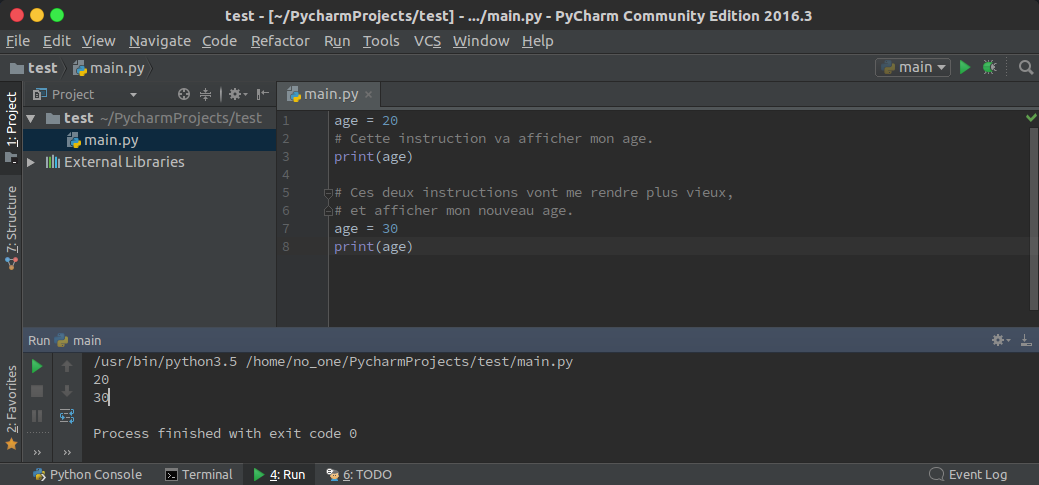
\includegraphics[width=\linewidth]{img/15_affiche_variables.png}
                \caption{Affichage de la variable age}
            \end{figure}

        \subsubsection{Quel genre d'information on peut stocker dans nos variable}
            Il existe essentiellement 3 types d'information qu'on peut stocker dans les variables :
            \begin{description}
                \item[Les entiers :] comme ce que nous avons stocké dans la variable \code{age} que nous avons 
                    utilisé jusque là. Les entiers sont appelé \code{int} en python.
                \item[Les valeurs décimales :] des nombres à virgules, (comme : 3.453). Ces nombres sont appelé 
                    \code{float} en python. Exemple :
                    \begin{lstlisting}[style=code]
pi = 3.14
                    \end{lstlisting}
                \item[Du texte :] on les appels les chaînes de caractères ou \code{string} en python. On les définit on les
                    entourant par \code{""} ou \code{''}. Exemple :
                    \begin{lstlisting}[style=code]
prenom = "Amine"
prenom2 = "Moustapha"
nom = 'Malaoui'
                    \end{lstlisting}
            \end{description}

        \subsubsection{Afficher les variables}
            Vous savez déjà qu'on peut afficher le contenu d'une variable avec \code{print()}, mais ce que vous 
            ne savez pas c'est que \code{print()} permet d'afficher plusieurs variables à la fois. Il suffit 
            juste de les séparer par des \code{,} :
            \begin{lstlisting}[style=code]
# Je cree mes variables
prenom = "Amine"
nom = "Malaoui"

print("Salut, je m'appelle", prenom, nom)
            \end{lstlisting}

            En exécutant notre programme, PyCharm nous affichera ça :

            \begin{lstlisting}[style=exec_result]
/usr/bin/python3.5 /home/no_one/PycharmProjects/test/main.py
Salut, je m'appelle Amine Malaoui

Process finished with exit code 0
            \end{lstlisting}

        \subsubsection{Récupérer une saisie}
            Ce que nous avons fait jusque là c'est de crée nos variables, et de les données des valeurs directement dans
            le code source. Ce que nous allons apprendre maintenant c'est de demander de l'utilisateur 
            de donner une valeur à notre variable au cours d'exécution.

            Pour cela on va utiliser l'instruction de récupération de saisie, qui est \code{input()} : 
            \begin{lstlisting}[style=code]
# On demande a l'utilisateur de nous donner son prenom,
# et on stock son prenom apres dans la variable prenom.
prenom = input("Veuillez entrer votre prenom : ")

# On dit bonjour a l'utilisateur.
print("Bonjour", prenom)
            \end{lstlisting}

            Ce que fait ce code c'est qu'il affiche à l'utilisateur \code{Veillez entrer votre prenom :}, et il lui 
            donne la main après pour qu'il entre son prénom. Son prénom est maintenant stocker dans la variable 
            \code{prenom}. Voila ce que PyCharm nous affiche après l'exécution :
            \begin{figure}[H]
                \centering
                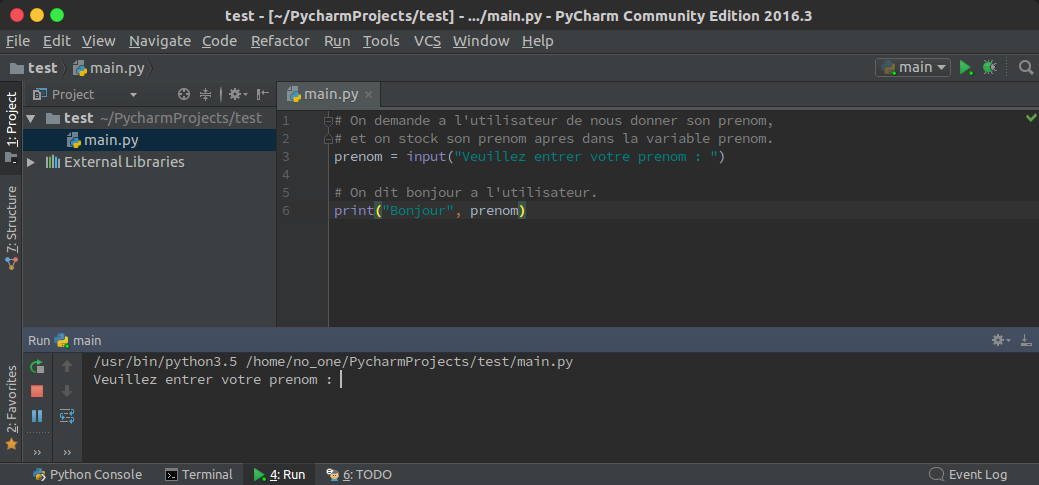
\includegraphics[width=\linewidth]{img/16_input.png}
                \caption{PyCharm attend qu'on entre le prénom}
            \end{figure}

            Dès que l'utilisateur entre son nom et tape \code{Entrée}, PyCharm lui affiche \code{Bonjour} suivi 
            du prénom de l'utilisateur :
            \begin{figure}[H]
                \centering
                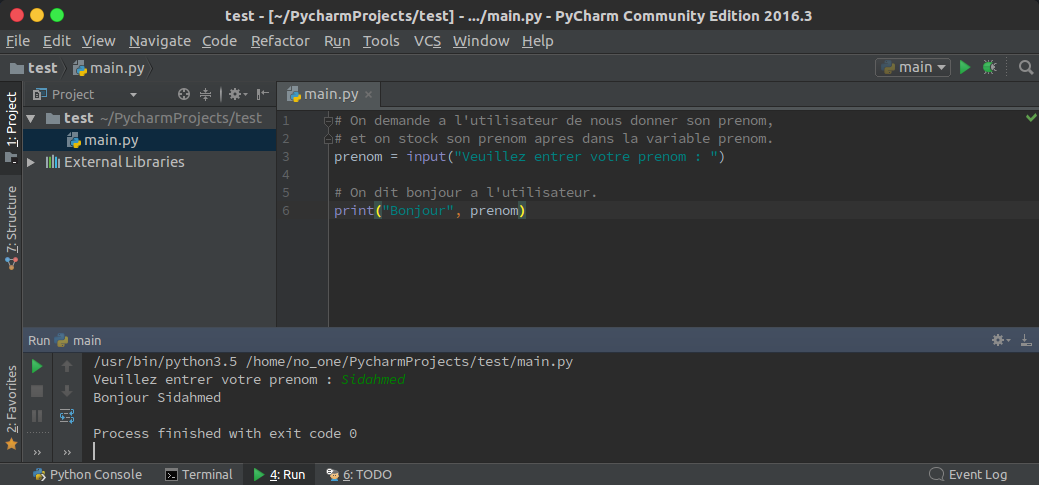
\includegraphics[width=\linewidth]{img/17_input.png}
                \caption{PyCharm affiche Bonjour suivi du prénom}
            \end{figure}

        \subsubsection{Comment nommé les variables}
            On va parler de la meilleur manière de nommé les variables avant de finir cette partie. 
            vous avez juste quelques règles à suivre, et tout passera à merveille :
            \begin{itemize}
                \item Le nom d'une variable doit commencer par une lettre. Exemple :
                    \begin{lstlisting}[style=code]
# Faux
1prenom = 20 

# Juste
prenom1 = 20 

# Juste
prenom = 20
                    \end{lstlisting}

                \item Donner toujours des noms explicites à vos variables. C'est à dire en observant le nom de votre
                    variable, il faut que vous serrez capable de comprendre son fonctionnement. Croyez moi, ça vous 
                    sera extrêmement utiles quand vous réexaminer votre code. \\Par exemple, si on veut stocker 
                    l'age d'un utilisateur :
                    \begin{lstlisting}[style=code]
# Faux, car c'est pas claire que x designe un age.
x = 20

# Juste
age = 20
                    \end{lstlisting}

                \item Si le nom de votre variable doit être composé de plusieurs mots, séparer les mots par un \code{\_}.
                    Exemple :
                    \begin{lstlisting}[style=code]
# Faux
notedemath = 15

# Juste
note_de_math = 15
                    \end{lstlisting}

                \item Et enfin, n'utilisez pas de caractères avec accents (comme \code{é}, \code{è}, \code{à} \ldots)
                    car ça peut vous posez des problèmes plus tard.
            \end{itemize}

            Enfin, nous avons terminé de parler sur les variables. Nous allons faire un petit exercices avant de passer
            à la section suivante.
        \subsubsection{Exercice 2}
            Ne sautez pas ces exercices, c'est très important de pratiquer en informatique.

            Voici l'énoncé de l'exercice :
            \begin{itemize}
                \item Créez un nouveau projet et nommé le ``exercice 2'', et créez un fichier ``main.py'' dans ce
                    projet.
                \item Débrouillez vous pour que le programme demande le ``prenom'', ``nom'' et ``age'' de l'utilisateur.
                    Puis affichez tous ça dans une phrase du genre : \code{Tu t'appelles Yanis Khelloufi et tu as 22 ans.}.
            \end{itemize}


\clearpage

    \subsection{les opérateurs arithmétique}
        Les ordinateurs sont des vrai machines à calcul, c'est ce qu'il savent faire le mieux. Donc dans cette partie
        nous allons apprendre à faire des calcules avec python.

        Il y a dans python 5 symboles qui nous permettent de faire des opérations arithmétique :
        \begin{itemize}
            \item \code{+} fait l'addition.
            \item \code{-} fait la soustraction.
            \item \code{*} fait la multiplication.
            \item \code{/} fait la division entière.
            \item \code{//} fait la division euclidienne.
            \item \code{\%} donne le reste de la division euclidienne (on appel ça le \emph{modulo}).
            \item \code{**} \colorbox{red}{fait la puissance.}
        \end{itemize}

        \subsubsection{Addition, soustraction, multiplication}
            Pour l'addition et la soustraction et la multiplication, rien de plus simple, on utilise seulement 
            les symboles approprié, et tout passe à merveille. Exemple :
            \begin{lstlisting}[style=code]
x = 10 + 5
y = 21 - 7
z = 9 * 9

# Ceci affichera : 15 14 81
print(x, y, z) 
            \end{lstlisting}

        \subsubsection{Division entière et Division euclidienne}
            Pour voir la différence, un exemple vaut mieux qu'un long discours :
            \begin{lstlisting}[style=code]
division_entiere = 10 / 3
division_euclidienne = 10 // 3

# Ceci affichera : 3.3333333333333335  3
print(division_entiere, division_euclidienne)
            \end{lstlisting}

        \subsubsection{Modulo (reste de la division euclidienne)}
            Exemple :
            \begin{lstlisting}[style=code, breaklines=false]
x = 10 % 3

# Ceci nous affichera 1. Car le reste de la division de 10 par 3 donne 1.
print(x) 
            \end{lstlisting}
        \subsubsection{La puissance}
            Rien de plus simple. Exemple :
            \begin{lstlisting}[style=code]
x = 5 ** 2

# Ceci affichera 125
print(x)
            \end{lstlisting}
        

        \subsubsection{Opérations entre variables}
            Sachez bien que toutes les opérations que nous avons vu précédemment sont aussi applicables sur les variables.
            Donc on peut faire des calculs entres variables. Exemple : 
            \begin{lstlisting}[style=code]
a = 10
b = 15
resultat = a + b

# Ceci affichera : 10 + 15 = 25
print(a, "+", b, "=", resultat)
            \end{lstlisting}

        \subsubsection{Un petit problème !}
            Essayez ce code : 
            \begin{lstlisting}[style=code, breaklines=false]

date_de_naissance = input("Veuillez entrez votre date de naissance : ")
age = 2017 - date_de_naissance

print("Votre avez", age, "ans")
            \end{lstlisting}

            Malheureusement, PyCharm n'a pas pu exécuter notre programme, et il nous affiche une erreur :
            \begin{lstlisting}[style=exec_result]
/usr/bin/python3.5 /home/no_one/PycharmProjects/test/main.py
Veuillez entrez votre date de naissance : 1994
Traceback (most recent call last):
  File "/home/no_one/PycharmProjects/test/main.py", line 3, in <module>
    age = 2017 - date_de_naissance
TypeError: unsupported operand type(s) for -: 'int' and 'str'

Process finished with exit code 1
            \end{lstlisting}

            Ce qui s'est passé c'est que l'instruction \code{input()} récupère la saisie sous forme de texte. Donc
            ce qu'elle a stocké dans la variable \code{date\_de\_naissance} n'est pas le nombre \code{1994} mais plutôt
            le texte (chaînes de caractères) \code{"1994"}. Donc quand Python arrive à l'instruction de la soustraction,
            il essaye de soustraire un texte d'un entier, et là ça plante, car ce n'est pas possible.

            La solution consiste à convertir notre variable \code{date\_de\_naissance} en un entier. C'est extrêmement 
            simple, il suffit juste d'utiliser l'instruction \code{int()}. Voici à quoi rassemblerai notre nouveau
            code source :
            \begin{lstlisting}[style=code, breaklines=false]
date_de_naissance = input("Veuillez entrez votre date de naissance : ")
# On converti notre variable en un entier.
date_de_naissance = int(date_de_naissance)

age = 2017 - date_de_naissance

print(age) 
            \end{lstlisting}

            Et cette fois, le programme marche à merveille. 

            N'oubliez pas, dorénavant, quand vous utilisez \code{input()},
            mettez en tête qu'elle récupère la saisie sous forme de texte. Pensez donc à convertir votre variable si 
            vous voulez l'utiliser comme entier (utilisez \code{int()}) ou nombre à virgule (utilisez \code{float()}).

        \subsubsection{Exercice 3}
            Voici l'énoncé de l'exercice :
            \begin{itemize}
                \item Créez un nouveau projet et nommé le ``exercice 3'', et créez un fichier ``main.py'' dans ce
                    projet.
                \item Demandez l'age de l'utilisateur, et dite lui à quel année il aura 100 ans.
            \end{itemize}
    \subsection{Les boucles}
        Explication des structures avec un exemple après chaque petite explication.
    \subsection{Découper le programme en fonctions}
        C'est quoi une fonction. Quelles sont les fonctions que nous avons déjà utilisés. Comment créer nos propres
        fonctions.
    \subsection{Les modules}
    \subsection{TP}
    \subsection{Le help}
        Obtenir le help depuis la console.

\section{La programmation orientée objet}
    \subsection{C'est quoi déjà un objet ?}
    \subsection{Les différents types d'objets disponible}
        On parlera des string, listes, tuples et des dictionnaires.
    \subsection{Les opérations sur les fichiers}
        Ouverture, lecture, écriture des fichiers.
    \subsection{Les chaînes de caractères}
    \subsection{Les listes}
    \subsection{Les tuples}
    \subsection{Les dictionnaires}
    \subsection{TP}

\section{Les bibliothèques standards}
    \subsection{Exécutions des commandes systèmes}
    \subsection{L'aléatoire}
    \subsection{Gestion des mots de passes}
    \subsection{Le réseau}

\section{Allez plus loin}
    Des tutos pour la programmation graphique avec PyQt. Le tuto d'openclassrooms.
\end{document}